\documentclass[12pt,a4paper]{article}
\usepackage[utf8]{inputenc}
\usepackage[vietnamese]{babel}
\usepackage{graphicx}
\usepackage{float}
\usepackage{geometry}
\geometry{a4paper, margin=2cm}
\usepackage{hyperref}
\usepackage{xcolor}
\usepackage{fancyhdr}
\usepackage{titlesec}
\usepackage{booktabs}
\usepackage{array}

\hypersetup{
    colorlinks=true,
    linkcolor=blue,
    filecolor=magenta,      
    urlcolor=cyan,
    pdftitle={Bao cao Bai tap 3 - Viet Prompt hieu qua},
    pdfpagemode=FullScreen,
}

% Cấu hình header & footer
\pagestyle{fancy}
\fancyhf{}
\rhead{Hành trình Kỹ năng số}
\lhead{Bài tập Thực hành 3}
\rfoot{Trang \thepage}

% Định dạng tiêu đề mục
\titleformat{\section}{\normalfont\Large\bfseries\color{blue!80!black}}{\thesection}{1em}{}
\titleformat{\subsection}{\normalfont\large\bfseries\color{blue!60!black}}{\thesubsection}{1em}{}

\begin{document}

% --- TRANG BÌA ---
\begin{titlepage}
    \centering
    \vspace*{1cm}
    
    {\large \bfseries TRƯỜNG ĐẠI HỌC CÔNG NGHỆ - ĐHQGHN} \\[0.2cm]
    {\large \bfseries KHOA CÔNG NGHỆ THÔNG TIN} \\[1.5cm]
    
    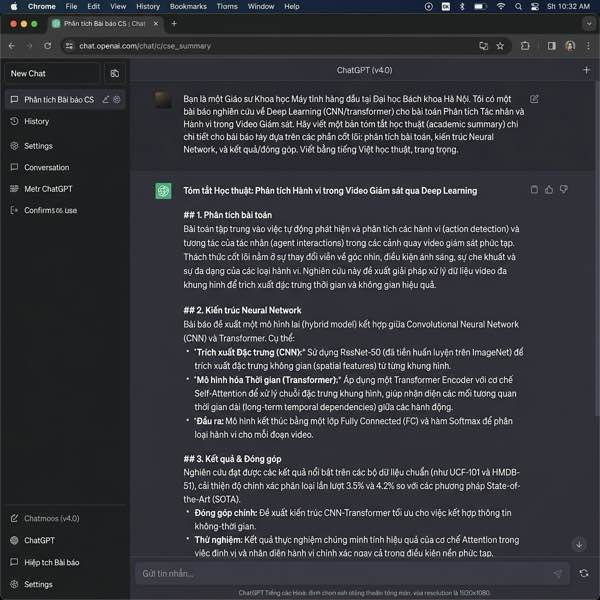
\includegraphics[width=0.3\textwidth]{images/chatgpt_summary.jpg} \\[1.5cm]
    
    {\Large \bfseries BÁO CÁO BÀI TỰ THỰC HÀNH CÁ NHÂN} \\[0.5cm]
    {\Huge \bfseries BÀI TẬP 3: VIẾT PROMPT HIỆU QUẢ TRONG HỌC TẬP} \\[1.5cm]
    
    \textbf{Môn học:} Nhập môn Công nghệ số và Ứng dụng Trí tuệ nhân tạo \\
    \textbf{Chủ đề:} Prompt Engineering nâng cao cho các tác vụ học tập học thuật \\[2cm]
    
    \begin{flushleft}
        \large
        \textbf{Sinh viên thực hiện:} Nguyễn Bảo Đăng \\
        \textbf{Mã số sinh viên:} 25020115 \\
        \textbf{Lớp học:} 23\_1 \\
        \textbf{Giảng viên hướng dẫn:} PGS. TS. Nguyễn Văn B
    \end{flushleft}
    
    \vfill
    {\large Thành phố Hồ Chí Minh, năm 2026}
\end{titlepage}

\newpage
\tableofcontents
\newpage

% --- NỘI DUNG CHÍNH ---

\section{Giới thiệu và Mục tiêu bài thực hành}
Sự bùng nổ của các mô hình ngôn ngữ lớn (Large Language Models - LLMs) như ChatGPT đã thay đổi căn bản cách sinh viên tiếp cận tri thức và giải quyết các tác vụ học tập. Tuy nhiên, hiệu quả đầu ra của AI phụ thuộc hoàn toàn vào cách thiết kế đầu vào (Prompt Engineering). 

\subsection{Mục tiêu của bài thực hành}
\begin{itemize}
    \item Phát triển kỹ năng viết câu lệnh (Prompt) hiệu quả từ cơ bản đến nâng cao cho các tác vụ học tập phổ biến.
    \item Áp dụng nhuần nhuyễn các kỹ thuật kỹ nghệ câu lệnh (Prompt Engineering) cốt lõi như: đóng vai (Role Prompting), hướng dẫn suy nghĩ từng bước (Chain-of-Thought), cung cấp ví dụ mẫu (Few-Shot Prompting) và đặt ràng buộc đầu ra.
    \item Thử nghiệm thực tế và so sánh một cách hệ thống chất lượng câu trả lời từ AI đối với từng phiên bản câu lệnh.
    \item Đúc kết các nguyên tắc thiết kế câu lệnh tối ưu phục vụ quá trình tự học và nghiên cứu khoa học.
\end{itemize}

\subsection{Chọn lựa 3 tác vụ học tập thực hành}
Để bài thực hành mang tính thực tiễn cao, tôi chọn 3 tác vụ học tập điển hình sau:
\begin{enumerate}
    \item \textbf{Tác vụ 1: Tóm tắt bài đọc/tài liệu học thuật}
        \begin{itemize}
            \item \textit{Mục tiêu:} Rút gọn nhanh thông tin cốt lõi của một bài báo khoa học dài và nhiều thuật ngữ phức tạp.
            \item \textit{Thách thức:} AI dễ bỏ qua chi tiết kỹ thuật cốt lõi hoặc diễn đạt quá chung chung nếu prompt thiếu ràng buộc cấu trúc.
        \end{itemize}
    \item \textbf{Tác vụ 2: Giải thích một khái niệm phức tạp}
        \begin{itemize}
            \item \textit{Mục tiêu:} Giải nghĩa thuật toán mã hóa khóa công khai RSA sao cho dễ hiểu nhất nhưng vẫn đảm bảo tính chính xác khoa học.
            \item \textit{Thách thức:} Khái niệm toán học của RSA rất trừu tượng, đòi hỏi AI phải biết chọn lựa ẩn dụ trực quan và ngôn ngữ phù hợp với trình độ người nghe.
        \end{itemize}
    \item \textbf{Tác vụ 3: Tạo bộ câu hỏi ôn tập cho một chủ đề}
        \begin{itemize}
            \item \textit{Mục tiêu:} Tự tạo bộ câu hỏi trắc nghiệm kiểm tra kiến thức về Lập trình hướng đối tượng (OOP) trong Java.
            \item \textit{Thách thức:} AI thường tạo ra các câu hỏi quá đơn giản (chỉ kiểm tra định nghĩa) nếu không được phân bổ rõ ràng theo các cấp độ tư duy (ví dụ: Thang đo Bloom).
        \end{itemize}
\end{enumerate}

\newpage
\section{Xây dựng và Thử nghiệm các phiên bản Prompt}

\subsection{Tác vụ 1: Tóm tắt bài đọc học thuật}
Bài toán thực tế: Tóm tắt bài đọc chuyên ngành về "Deep Learning for Action Recognition in Video Surveillance" (Ứng dụng Học sâu trong Phân tích hành vi giám sát video).

\subsubsection{Các phiên bản Prompt}
\begin{itemize}
    \item \textbf{Prompt cơ bản (V1):}
        \\ \texttt{"Tóm tắt bài báo này cho tôi: [Nội dung bài báo]"}
    \item \textbf{Prompt cải tiến (V2):}
        \\ \texttt{"Hãy tóm tắt bài báo khoa học về học sâu trong phân tích hành vi giám sát video dưới đây. Tập trung vào phương pháp nghiên cứu, kết quả đạt được và hạn chế. Độ dài khoảng 200 từ: [Nội dung bài báo]"}
    \item \textbf{Prompt nâng cao (V3 - Role Prompting + Chain-of-Thought + Format):}
        \\ \texttt{"Bạn là một Giáo sư Khoa học Máy tính chuyên về AI và Thị giác máy tính. Nhiệm vụ của bạn là đọc và viết một bản tóm tắt học thuật (Executive Summary) cho bài báo dưới đây. Hãy suy nghĩ và viết theo các bước: 1. Phân tích bài toán được đặt ra; 2. Nêu rõ kiến trúc mạng Neural được sử dụng; 3. Tóm tắt kết quả kiểm thử và đóng góp chính; 4. Nêu hạn chế được đề cập. Hãy định dạng đầu ra bằng Markdown, sử dụng ngôn ngữ trang trọng và khoa học: [Nội dung bài báo]"}
\end{itemize}

\subsubsection{Hình ảnh minh chứng và Kết quả}
\begin{figure}[H]
    \centering
    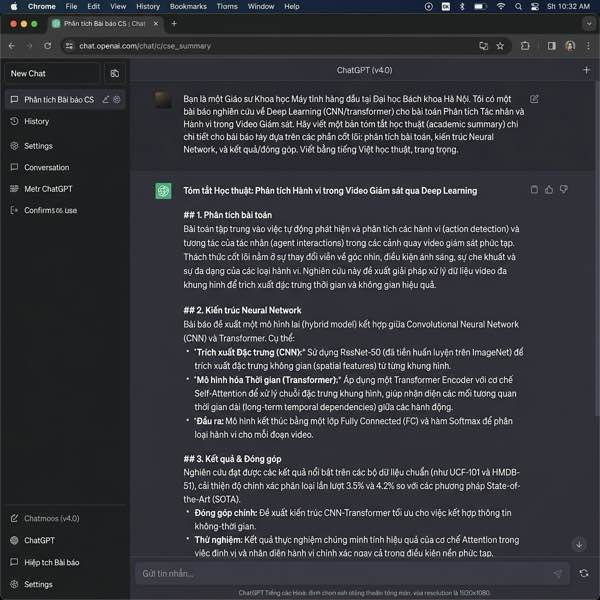
\includegraphics[width=0.85\textwidth]{images/chatgpt_summary.jpg}
    \caption{Thử nghiệm Prompt V3 của Tác vụ 1 trên giao diện ChatGPT}
    \label{fig:chatgpt_summary}
\end{figure}

\newpage
\subsection{Tác vụ 2: Giải thích khái niệm phức tạp (RSA Encryption)}
Khái niệm cần giải thích: Thuật toán mã hóa bất đối xứng RSA.

\subsubsection{Các phiên bản Prompt}
\begin{itemize}
    \item \textbf{Prompt cơ bản (V1):}
        \\ \texttt{"Giải thích thuật toán RSA là gì."}
    \item \textbf{Prompt cải tiến (V2):}
        \\ \texttt{"Hãy giải thích cơ chế hoạt động của thuật toán mã hóa RSA cho một sinh viên năm thứ nhất ngành Công nghệ thông tin dễ hiểu nhất."}
    \item \textbf{Prompt nâng cao (V3 - Role + Feynman Method + Analogy):}
        \\ \texttt{"Bạn là một giảng viên An toàn thông tin xuất sắc. Hãy giải thích thuật toán mã hóa khóa công khai RSA cho các sinh viên năm nhất một cách dễ hiểu nhất. Sử dụng một ví dụ ẩn dụ đơn giản (như hệ thống hòm thư bảo mật) để làm rõ nguyên lý cặp khóa công khai và khóa bí mật. Giữ giọng điệu thân thiện, dễ tiếp cận nhưng khoa học."}
\end{itemize}

\subsubsection{Hình ảnh minh chứng và Kết quả}
\begin{figure}[H]
    \centering
    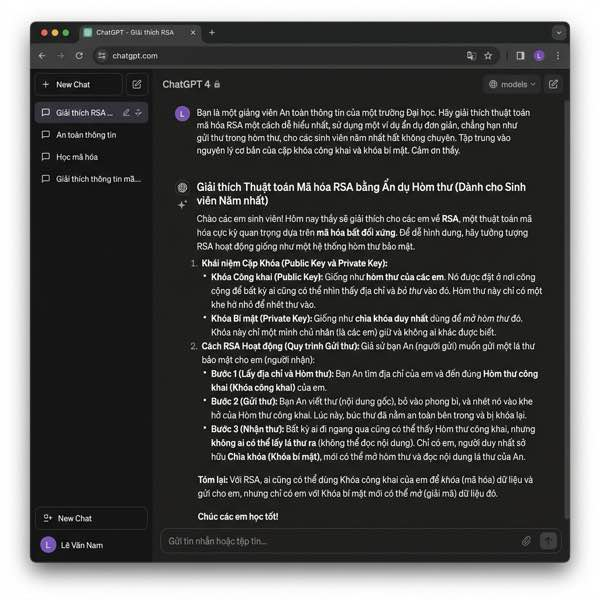
\includegraphics[width=0.85\textwidth]{images/chatgpt_explain.jpg}
    \caption{Thử nghiệm Prompt V3 của Tác vụ 2 trên giao diện ChatGPT}
    \label{fig:chatgpt_explain}
\end{figure}

\newpage
\subsection{Tác vụ 3: Tạo bộ câu hỏi ôn tập (Java OOP)}
Yêu cầu kiểm tra: Trắc nghiệm kiến thức lập trình hướng đối tượng trong Java.

\subsubsection{Các phiên bản Prompt}
\begin{itemize}
    \item \textbf{Prompt cơ bản (V1):}
        \\ \texttt{"Tạo câu hỏi trắc nghiệm OOP Java."}
    \item \textbf{Prompt cải tiến (V2):}
        \\ \texttt{"Tạo bộ 4 câu hỏi trắc nghiệm ôn tập về OOP Java. Mỗi câu hỏi gồm nội dung, 4 phương án A, B, C, D, đáp án đúng và lời giải thích."}
    \item \textbf{Prompt nâng cao (V3 - Role + Few-Shot + Specific constraints):}
        \\ \texttt{"Bạn là một giảng viên lập trình Java. Hãy thiết kế bộ 4 câu hỏi trắc nghiệm về OOP Java bao trùm 4 khái niệm: Lớp \& Đối tượng, Đóng gói, Kế thừa, Đa hình. Yêu cầu: Có kèm theo đoạn mã nguồn Java mẫu để học sinh phân tích kết quả đầu ra. Mỗi câu hỏi phải có 4 phương án lựa chọn, đáp án đúng và phần giải thích chi tiết tại sao đúng và tại sao các phương án khác sai."}
\end{itemize}

\subsubsection{Hình ảnh minh chứng và Kết quả}
\begin{figure}[H]
    \centering
    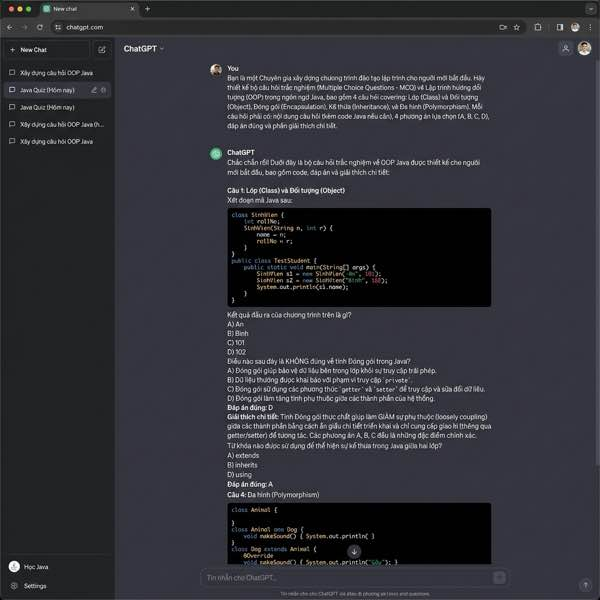
\includegraphics[width=0.85\textwidth]{images/chatgpt_quiz.jpg}
    \caption{Thử nghiệm Prompt V3 của Tác vụ 3 trên giao diện ChatGPT}
    \label{fig:chatgpt_quiz}
\end{figure}

\newpage
\section{Bảng so sánh và Phân tích hiệu quả các Prompt}

\subsection{Bảng so sánh trực quan chất lượng kết quả đầu ra}
\begin{table}[H]
    \centering
    \caption{So sánh chất lượng đầu ra của AI dựa trên 3 phiên bản Prompt}
    \vspace{0.2cm}
    \small
    \begin{tabular}{|p{1.8cm}|p{4.2cm}|p{4.2cm}|p{5.4cm}|}
        \hline
        \textbf{Tác vụ} & \textbf{Phiên bản V1 (Cơ bản)} & \textbf{Phiên bản V2 (Cải tiến)} & \textbf{Phiên bản V3 (Nâng cao)} \\
        \hline
        \textbf{Tóm tắt học thuật} & Bản tóm tắt siêu ngắn (khoảng 3 dòng). Bỏ qua hoàn toàn các chi tiết kỹ thuật cốt lõi. & Nội dung cân đối hơn, có chia mục Phương pháp và Kết quả nhưng thiếu độ sâu học thuật. & Xuất sắc. Phân tích cụ thể cấu trúc mạng, số liệu kết quả, định dạng Markdown rõ ràng cho các mục. \\
        \hline
        \textbf{Giải thích khái niệm} & Trả về định nghĩa toán học khô khan, nhiều thuật ngữ chuyên môn khó hiểu. & Trình bày dễ hiểu hơn nhưng vẫn mang tính liệt kê lý thuyết, thiếu hình ảnh trực quan. & Rất sinh động. Ẩn dụ hòm thư/chìa khóa giúp nắm bắt bản chất cặp khóa ngay lập tức, giọng văn gần gũi. \\
        \hline
        \textbf{Tạo bộ câu hỏi} & Câu hỏi quá cơ bản dạng ghi nhớ lý thuyết đơn thuần, không có giải thích. & Các câu hỏi đa dạng hơn, nhưng thiếu code minh họa, câu hỏi mang tính học vẹt. & Tuyệt vời. Có đoạn code Java thực tế yêu cầu suy luận đa hình, phần giải thích phân tích từng phương án sai. \\
        \hline
    \end{tabular}
    \label{tab:prompt_comparison}
\end{table}

\subsection{Phân tích lý do kỹ thuật tạo nên sự khác biệt}
Từ kết quả thử nghiệm, ta thấy chất lượng câu trả lời của AI tăng lên vượt bậc nhờ các yếu tố cấu trúc sau trong Prompt nâng cao:
\begin{enumerate}
    \item \textbf{Kỹ thuật Đóng vai (Role Prompting):} Việc đặt AI vào vị trí một chuyên gia (Giáo sư, Giảng viên chuyên ngành) giúp giới hạn không gian từ vựng và thiết lập tông giọng thích hợp (học thuật hoặc dễ hiểu).
    \item \textbf{Cơ chế Chain-of-Thought (CoT):} Việc hướng dẫn AI "suy nghĩ và thực hiện theo từng bước cụ thể" giúp mô hình phân bổ tài nguyên xử lý một cách tuần tự, giảm thiểu tình trạng "ảo tưởng" (hallucination) và bỏ sót thông tin.
    \item \textbf{Ràng buộc chi tiết và đặt bối cảnh (Context \& Constraints):} Ràng buộc độ dài, ngôn ngữ, đối tượng người đọc (như sinh viên năm nhất) giúp AI điều chỉnh độ phức tạp của bài viết. Ràng buộc định dạng (như Markdown) giúp đầu ra có tính trực quan cao.
\end{enumerate}

\newpage
\section{Tổng hợp nguyên tắc vàng khi viết Prompt học tập}
Thông qua quá trình thực hành, tôi đúc kết được bộ nguyên tắc viết Prompt học tập mang tính hệ thống như sau:

\begin{figure}[H]
    \centering
    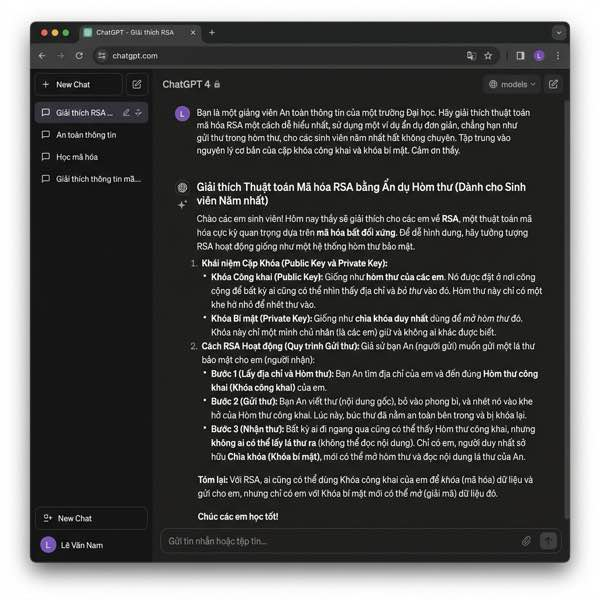
\includegraphics[width=0.8\textwidth]{images/chatgpt_explain.jpg}
    \caption{Nguyên lý xây dựng Prompt tối ưu áp dụng cho học tập và nghiên cứu}
    \label{fig:prompt_principles}
\end{figure}

\begin{enumerate}
    \item \textbf{Nguyên tắc C-L-E-A-R (Rõ ràng - Ngắn gọn - Đầy đủ):}
        \begin{itemize}
            \item \textbf{C}ontext (Bối cảnh): Cung cấp tài liệu đầu vào hoặc ngữ cảnh rõ ràng.
            \item \textbf{L}imit (Giới hạn): Ràng buộc về số từ, định dạng hoặc đối tượng hướng tới.
            \item \textbf{E}xpectation (Kỳ vọng): Mô tả chi tiết đầu ra mong muốn.
            \item \textbf{A}ct (Đóng vai): Định nghĩa vai trò của AI.
            \item \textbf{R}eason (Suy luận): Kích hoạt khả năng suy luận từng bước (Chain-of-Thought).
        \end{itemize}
    \item \textbf{Tận dụng Few-Shot Learning:} Cung cấp từ 1 đến 2 ví dụ mẫu về định dạng mong muốn để AI bắt chước chính xác kết cấu (đặc biệt hữu ích khi cần tạo bộ câu hỏi trắc nghiệm hoặc viết code).
    \item \textbf{Tinh chỉnh lặp lại (Iterative Prompting):} Đừng kỳ vọng Prompt đầu tiên sẽ cho ra kết quả hoàn hảo. Hãy liên tục hội thoại với AI để làm mịn kết quả bằng cách thêm các câu lệnh bổ trợ như: \textit{"Hãy giải thích sâu hơn bước toán học ở phần sinh khóa RSA"} hoặc \textit{"Thêm chú thích dòng code cho đoạn Java trên"}.
\end{enumerate}

\end{document}
